\section{Method}
\label{sec:methodology}

\begin{figure*}[h!]
	\centering
	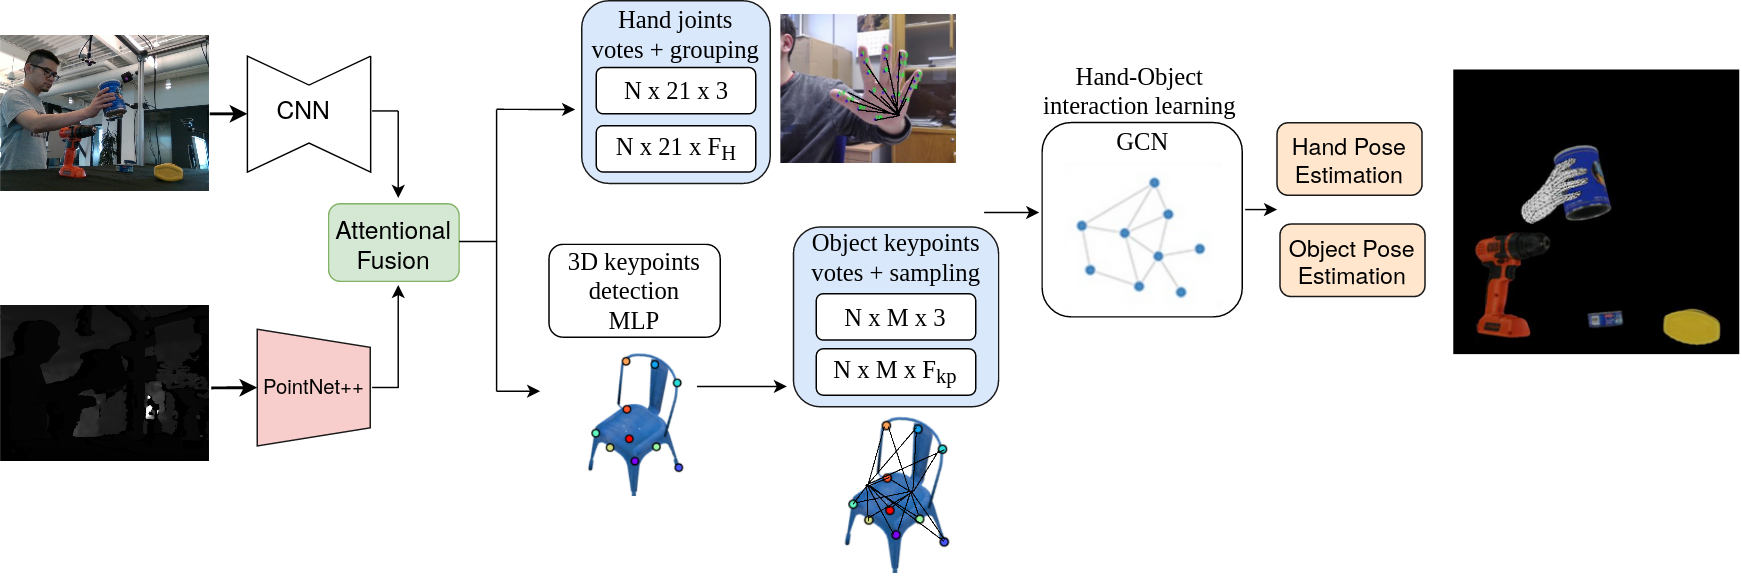
\includegraphics[width=0.95\linewidth]{Figs/Hand-Object_pose.png}
	\caption{Overview of our proposal. Our method takes both color and depth maps as input data. The color features are extracted by a CNN, while the 3D features are calculated by PointNet++ architecture. These two types of features are then fused together at pixel-level to obtain the new distinctive features. The attention mechanism is applied for the such new features to learn the contribution disparity of the context to the hand pose. The votes are computed and then regressed to estimate the MANO parameters.}
	\label{fig:Hand pose}
\end{figure*}

In Figure \ref{fig:Hand pose}, we provide an overall pipeline of our method for 3D hand mesh estimation. Our proposed network consists of backbone, Attention, voting and cluster and hand pose Estimation.

\subsection{Feature Extraction and Attentional Fusion}
\label{sec:data fusion}
Given a color map $I_{rgb} \in \mathbb{R}^{H \times W \times 3}$, the color features $f_{rgb} = \{ f^{rgb}_i \} ^{H \times W}_{i=1}$ are normally extracted by a CNN architecture. Where $f_{rgb} \in \mathbb{R}^{H \times W \times d_{rgb}}$ and each pixel is mapped into a color feature space $f^{rgb}_i \in \mathbb{R}^{d_{rgb}}$. The geometric features, on the other hand, are extracted by converting depth maps to point cloud and then feeding into PointNet \cite{qi2017pointnet}. In our work, differing from the original work, we conduct PointNet++ \cite{qi2017pointnet++}, an upgraded version, to replace the original backbone. Moreover, instead of only extracting the 3D point cloud feature of points inside the segmented region, our method applies the whole depth map without requiring semantic segmentation as in DenFusion. However, most of the pixels and points are background, which is redundant and harms hand pose estimation. We overcome this problem by adding an attention model to find out where should pay more attention to. Given a depth map $I_d \in \mathbb{R}^{H \times W \times 1}$, the point cloud features $f_{geo} = \{f^{geo}_i\}^{H \times W}_{i=1}$. Where $f_{geo} = \in \mathbb{R} ^{H \times W \times d_{geo}}$ and point cloud pixel at each position is $f^{geo}_i \in \mathbb{R}^{d_{geo}}$.

\begin{equation}
	f_i = A \times f^{rgb}_i \oplus B \times f^{geo}_i \
\end{equation}

\subsection{Hand and Object Voting}
\label{sec:voting}


\subsection{Hand-Object Interation Learning}
\label{sec:interaction}
